\documentclass{article}
\usepackage{graphicx}
\usepackage{wrapfig}
\usepackage{float}
\usepackage{geometry}
\geometry{
 a4paper,
 total={170mm,257mm},
 left=20mm,
 top=20mm,
 }

\begin{document}
\date{\today}
\author{Mark Samuel (202201857)}
\title{Assignment 01 \\ 
        \large Reinforcement Learning }
\maketitle

\section{Paper Based}

\subsection{Question 01}
\subsubsection{Symbol Definition}
\large Status:

\begin{equation}
    Appreciating \rightarrow A
\end{equation}

\begin{equation}
    Depreciating \rightarrow D
\end{equation}

\begin{equation}
    Stable \rightarrow S
\end{equation}

\subsubsection{Transition Matrix}
\begin{table}[h!]
    \centering
    \begin{tabular}{|c | c | c | c|}
        \hline
        Current | next & A & D & S\\ 
        \hline
        A & 25\% & 40\% & 35\% \\
        D & 30\% & 50\% & 20\% \\
        S & 33.333\% & 33.333\% & 33.333\% \\
        \hline
    \end{tabular}
    \caption{Transition Matrix of Question 1}
    \label{q1_Transition_matrix}
\end{table}

\subsubsection{Markov Chain}
The previous Transition Matrix can be modeled as Markov chain as in Figure \ref{q1_markovChain}
\begin{figure}[H]
    \centering
    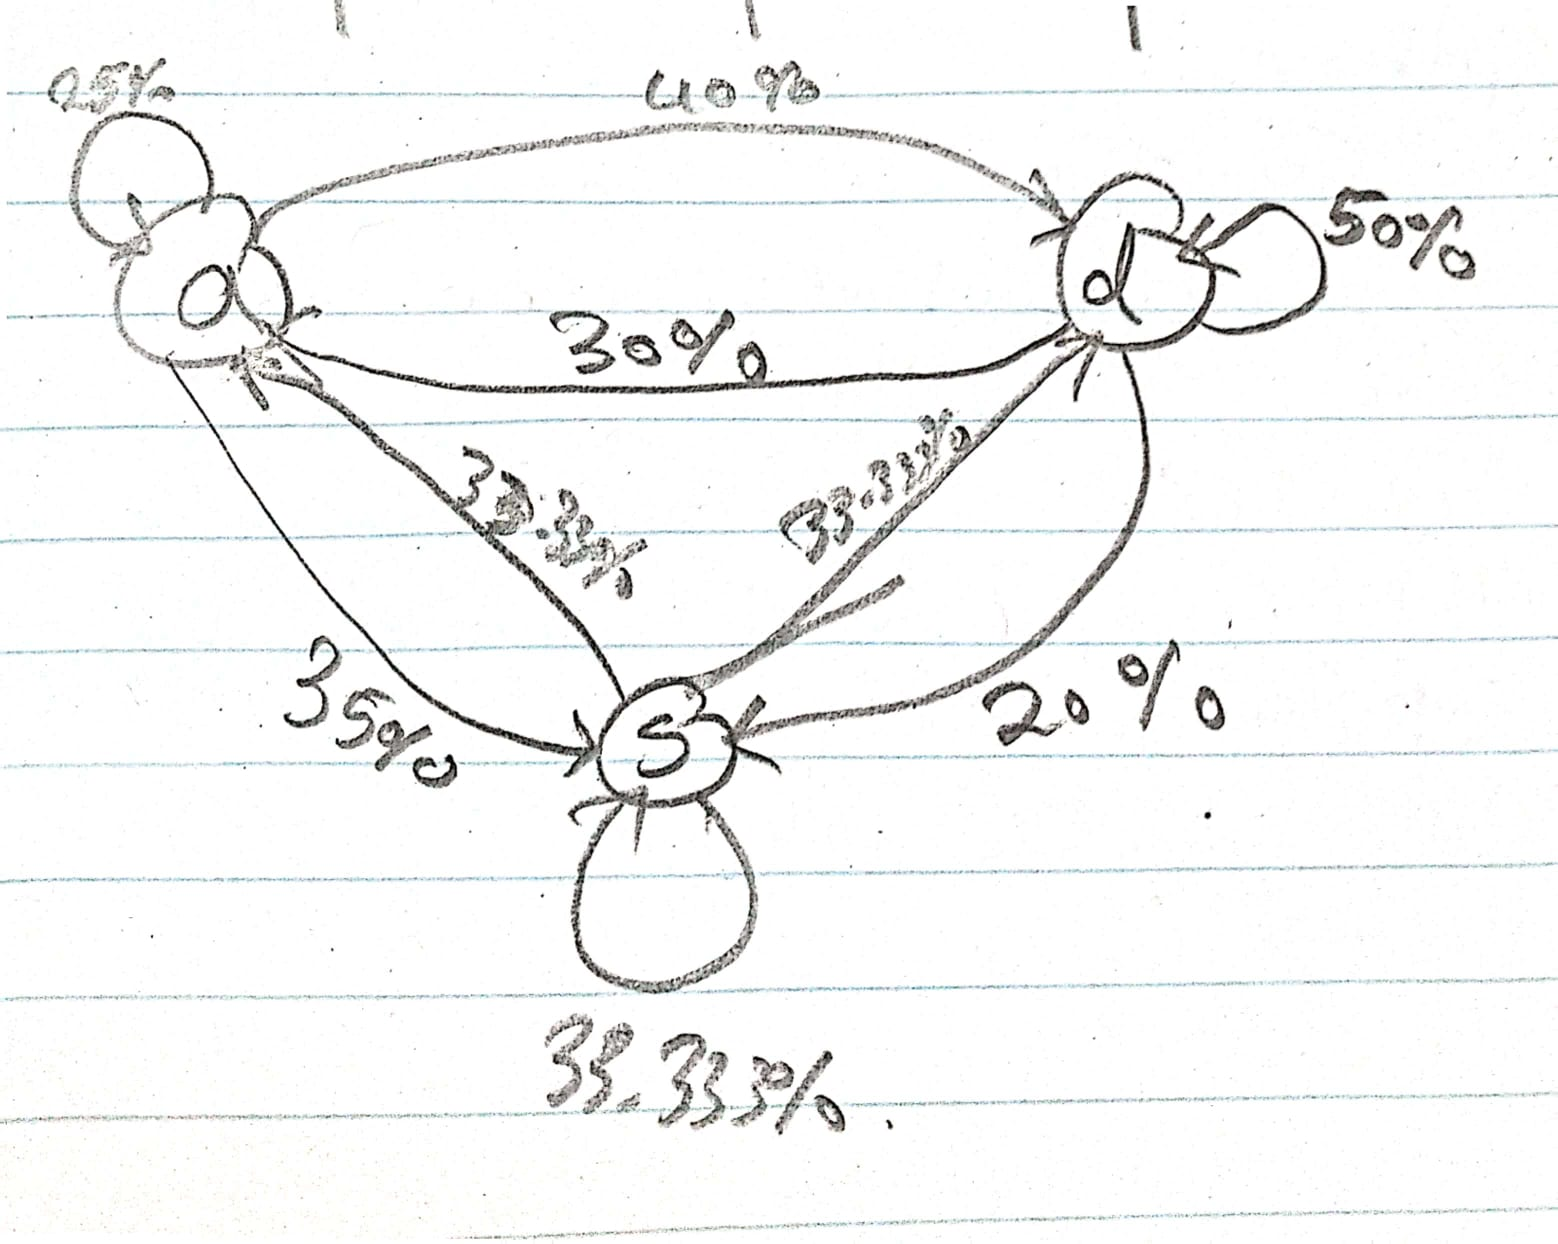
\includegraphics[width=.5\linewidth]{q1 chain.jpg}
        \caption{Markov Chain Handwritten}

    \label{q1_markovChain}
\end{figure}
\subsection{Question 02}
\subsubsection{Transition Matrix}
As defined in \ref{q2_Transition_matrix}
\begin{table}[h!]
    \centering
    \begin{tabular}{|c | c | c | c| c|}
        \hline
        Current | next & 1 & 2 & 3 & 4\\ 
        \hline
        1 & 25\% & 35\% & 40\% & 0\%\\
        2 & 55\% & 0\% & 0\% & 45\%\\
        3 & 0\% & 20\% & 60\%& 20\% \\
        4 & 30\% & 30\% & 20\% & 20\%\\
        \hline
    \end{tabular}
    \caption{Transition Matrix of Question 2}
    \label{q2_Transition_matrix}
    
\end{table}
\subsubsection{Written Question}
\begin{enumerate}
    \item {20\%}
    \item {25\%}
    \item {60\%}
\end{enumerate}

\section{Implementation}
\subsection{Transition Matrix}
The transition matrix is as defined as in transition Table \ref{q2_Transition_matrix}
\subsection{After Large number of Transitions}
\begin{table}[H]
    \centering
    \begin{tabular}{|c | c | c | c| c|}
        \hline
        Current | next & 1 & 2 & 3 & 4\\ 
        \hline
      1 & 23.89827 & 21.35726 & 34.17216 & 20.57231 \\
      2 & 23.88496 & 21.38767 & 34.18412 & 20.54325 \\
      3 & 23.89613 & 21.36379 & 34.17396 & 20.56612 \\
      4 & 23.89642 & 21.36231 & 34.17426 & 20.56701 \\
        \hline
    \end{tabular}
    \caption{Transition Matrix after 3 Transitions}
    \label{q2_Transition_matrix_many_transitions}
    
\end{table}
\subsection{Implementation in Networkx}
Kindly take a look at the file main.py and the graph is in figure \ref{q2_markovChain_python}
\begin{figure}[H]
    \centering
    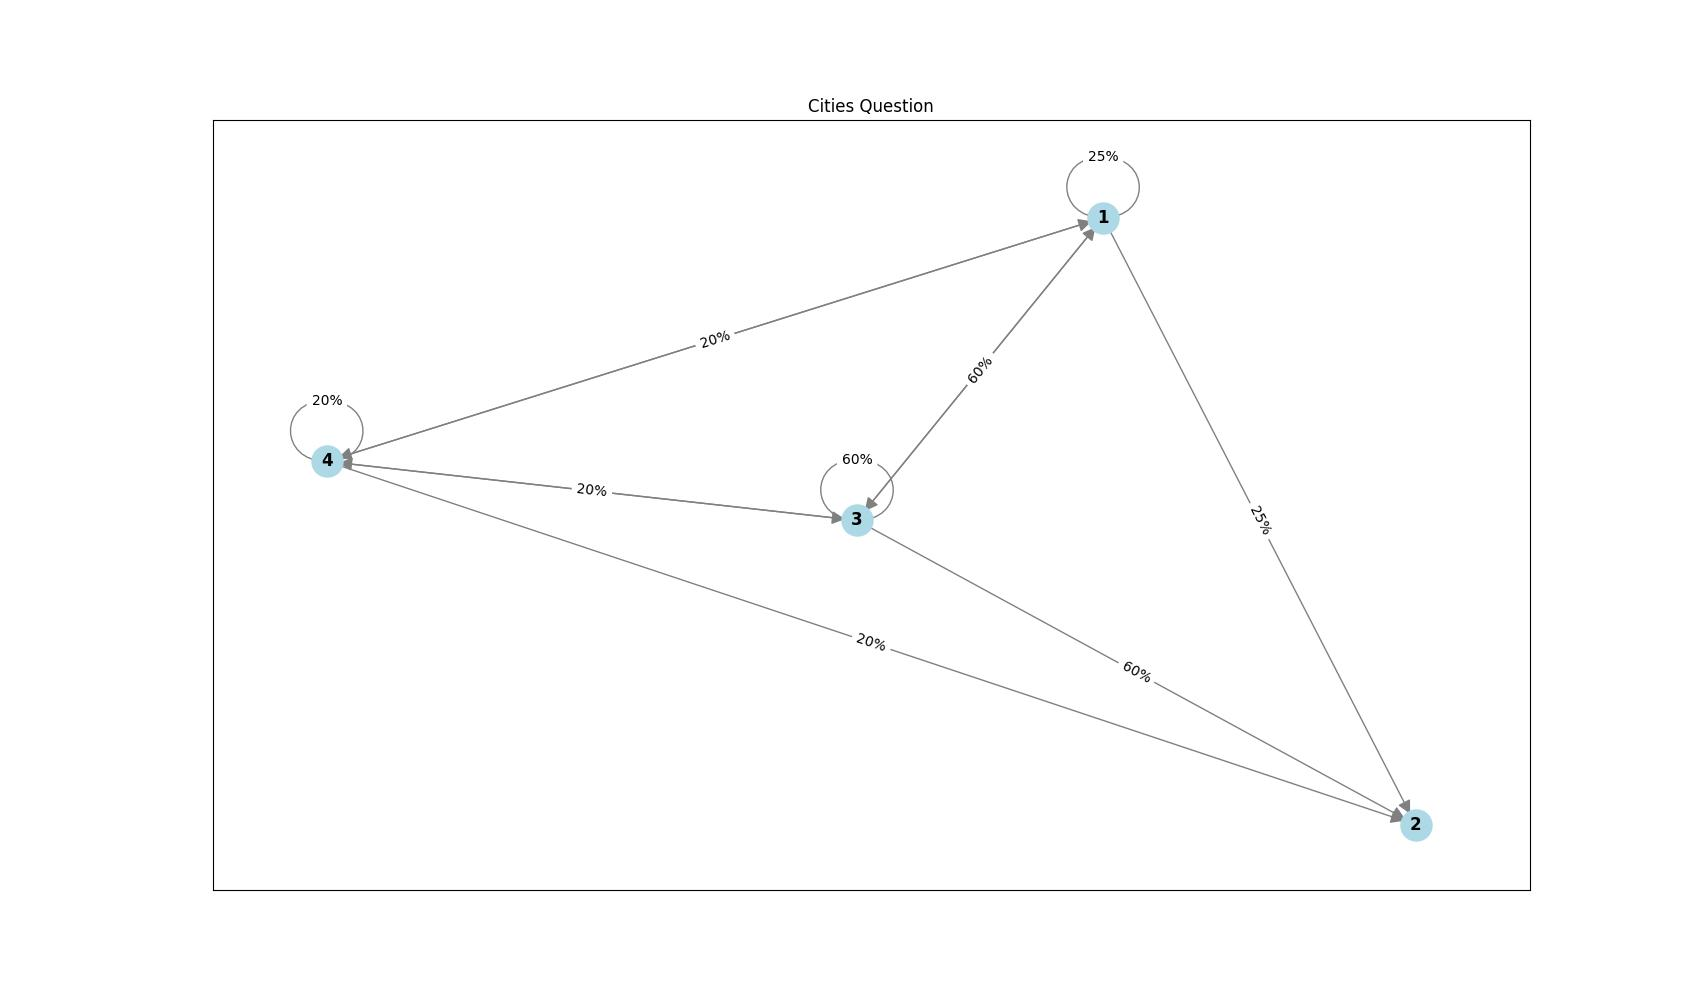
\includegraphics[width=\linewidth]{nodes.jpg}
        \caption{Implementation of the graph of Question 1}

    \label{q2_markovChain_python}
\end{figure}
\end{document}